\documentclass[11pt]{report}
\usepackage[a4paper,margin=1in]{geometry}
\usepackage[T1]{fontenc}
\usepackage[utf8]{inputenc}
\usepackage{lmodern}
\usepackage{microtype}
\usepackage{setspace}
\usepackage{xcolor}
\usepackage{booktabs}
\usepackage{array}
\usepackage{tabularx}
\usepackage{longtable}
\usepackage{multirow}
\usepackage{caption}
\usepackage{subcaption}
\usepackage{graphicx}
\usepackage{float}
\usepackage{hyperref}
\usepackage{enumitem}
\usepackage{pgfplots}
\usepackage{pgf-pie}
\usepackage{tikz}
\usetikzlibrary{positioning,arrows.meta}
\pgfplotsset{compat=1.18}
\hypersetup{colorlinks=true,linkcolor=blue!50!black,urlcolor=blue!50!black,citecolor=blue!50!black}
\onehalfspacing

\definecolor{navy}{HTML}{12344D}
\definecolor{teal}{HTML}{0F766E}
\definecolor{amber}{HTML}{B45309}
\definecolor{brick}{HTML}{B91C1C}
\definecolor{blueaccent}{HTML}{2563EB}
\definecolor{slate}{HTML}{64748B}
\definecolor{greenaccent}{HTML}{15803D}
\definecolor{softbg}{HTML}{F7FAFC}
\definecolor{rulegray}{HTML}{6B7280}
\definecolor{sarsaorange}{HTML}{C2410C}

\newcommand{\QL}{\textbf{Q-Learning}}
\newcommand{\SARSA}{\textbf{SARSA}}
\newcommand{\Bandit}{\textbf{Bandit}}
\newcommand{\Rule}{\textbf{Rule}}
\newcommand{\KMeans}{\textbf{K-Means}}
\newcommand{\TT}{\textbf{Train-Ticket}}
\newcommand{\TS}{\textbf{Timescale OpenTelemetry Demo}}
\newcommand{\SP}{\textbf{Spring Petclinic Microservices}}
\newcommand{\best}[1]{\textbf{#1}}

\setlist[itemize]{leftmargin=1.5em}
\setlength{\parindent}{0pt}
\setlength{\parskip}{0.5em}

\begin{document}

\begin{titlepage}
    \centering
    \vspace*{2cm}
    {\Huge\bfseries Final RQ1 Report Across Three Microservice Applications\par}
    \vspace{0.6cm}
    {\Large Adaptive Tracing with RL and Non-RL Controllers\par}
    \vspace{1.4cm}
    {\large Train-Ticket, Timescale OpenTelemetry Demo, and Spring Petclinic Microservices\par}
    \vspace{2cm}
    \begin{tabular}{rl}
        \textbf{Research question:} & How does RL-based adaptive tracing compare to non-RL baselines \\
        & when both are evaluated under the same system and runtime conditions? \\
        \textbf{Methods compared:} & Q-Learning, SARSA, Bandit, Rule, K-Means \\
        \textbf{Scenarios:} & Healthy and Faulted \\
        \textbf{Action space:} & Sampling rates $\{0.05, 0.10, 0.20, 0.50, 0.80\}$ \\
        \textbf{Generated:} & April 7, 2026 \\
    \end{tabular}
    \vfill
    {\large Consolidated LaTeX report generated from the final per-system RQ1 reports and experiment outputs.\par}
\end{titlepage}

\tableofcontents
\clearpage

\chapter*{Abstract}
\addcontentsline{toc}{chapter}{Abstract}
This report answers RQ1 across three different microservice applications: \TT, \TS, and \SP. The study compares three RL-based adaptive tracing controllers (\QL, \SARSA, and \Bandit) against two non-RL baselines (\Rule{} and \KMeans{}). In all three applications, the controller action is the tracing sampling rate, and the comparison is carried out under both healthy and faulted conditions. The combined result is not a universal RL win. Instead, the evidence shows a stronger and more defensible conclusion: RL-based adaptive tracing is consistently competitive, often strong, and sometimes clearly superior, but the best method remains application-dependent. \QL is strongest overall on \TT, \Rule{} achieves the best final latency on \TS, and \Bandit{} is strongest on final runtime metrics in \SP. This makes the main answer to RQ1 clear: RL-based adaptive tracing is a credible and often high-performing choice, but there is no single controller that dominates all systems.

\chapter{Research Question and Scope}
\section{Research question}
The report addresses the following question:

\textbf{RQ1:} \emph{How does RL-based adaptive tracing compare to non-RL adaptive tracing baselines, such as rule-based and clustering-based methods, when all methods are evaluated under the same microservice system and the same runtime conditions?}

The key point is methodological fairness. Each controller is evaluated inside the same application, under the same traffic conditions, using the same action space and the same observation model. The report is therefore not about whether one algorithm wins one benchmark once. It is about whether the RL family retains an advantage when the comparison is repeated across three different applications with different telemetry pipelines, service topologies, and degradation behavior.

\section{Why this comparison matters}
Fixed-rate tracing is easy to deploy, but it is a poor fit for dynamic systems. If the rate is too high, overhead increases unnecessarily. If the rate is too low, diagnostic visibility drops at the point where visibility is most needed. Adaptive tracing makes the rate a control decision rather than a constant. That decision can be made by:
\begin{itemize}
    \item \textbf{RL-based methods}, which learn or estimate the value of tracing actions from experience; or
    \item \textbf{Non-RL baselines}, which use explicit thresholds or clustering logic.
\end{itemize}
The practical question is whether RL adds enough value to justify its added complexity.

\chapter{Concepts, Methods, and Evaluation Terms}
\section{Adaptive tracing}
Adaptive tracing changes the trace sampling rate at runtime. Higher sampling gives more observability but increases data volume and overhead. Lower sampling reduces overhead but risks missing important traces. In this study, every controller selects from the same discrete action space: $0.05$, $0.10$, $0.20$, $0.50$, and $0.80$.

\section{Healthy and faulted scenarios}
\textbf{Healthy} means the application is operating under its normal workload and service behavior. \textbf{Faulted} means the runtime condition is intentionally degraded. The fault mechanism is application-specific: this is necessary because the systems do not expose identical fault mechanisms. What matters for RQ1 is that each application is compared internally under a normal and a degraded condition.

\section{Measured outputs}
The comparison uses the following runtime signals:
\begin{itemize}
    \item \textbf{Latency:} average request or trace latency. Lower is better.
    \item \textbf{QPS:} throughput in queries per second or an equivalent interval throughput measure. Higher is better.
    \item \textbf{Error rate:} the fraction of requests or traces marked as failed.
    \item \textbf{Trace total:} the amount of captured telemetry during a decision window or experiment run.
    \item \textbf{Average reward:} RL-specific scalar feedback used by learning-based controllers.
\end{itemize}
Reward is useful, but it is not always the strongest indicator of runtime quality. In particular, the \TS{} reward design is not a pure performance score, so latency, QPS, and error rate are treated as stronger evidence there.

\section{Controller families}
\subsection{RL-based methods}
\begin{itemize}
    \item \QL{} is an \emph{off-policy temporal-difference} method. It estimates long-run action value independently of the exact next action taken by the current behavior policy.
    \item \SARSA{} is an \emph{on-policy temporal-difference} method. It updates using the next action actually chosen by the current policy, which often makes it more conservative than Q-Learning.
    \item \Bandit{} is a simpler action-value controller. It focuses on the immediate payoff of tracing actions without learning a fuller state-transition structure.
\end{itemize}

\subsection{Non-RL baselines}
\begin{itemize}
    \item \Rule{} is a heuristic threshold-based controller. It uses explicit runtime logic rather than learned value estimates.
    \item \KMeans{} is a clustering-based baseline. It groups observed runtime states and maps each cluster to a tracing rate.
\end{itemize}

\chapter{Applications Under Study}
\section{Train-Ticket}
\TT{} is a railway ticket booking benchmark with a richer multi-service interaction pattern than the other applications in the study. It is the most mature experimental environment in the project and provides the strongest evidence set for RQ1. The final results on this application are stable, the number of decisions is high, and the policy comparison is the most defensible.

\section{Timescale OpenTelemetry Demo}
\TS{} is a lightweight password-generator application where a generator service fans out to upper, lower, digit, and special services. It is smaller than \TT{}, but still produces genuine distributed traces. The telemetry pipeline is strong and explicit: OpenTelemetry Collector, Promscale, TimescaleDB, Jaeger, and Grafana. This makes it a useful second application because it preserves real tracing behavior while remaining lightweight enough to run locally.

\section{Spring Petclinic Microservices}
\SP{} is a realistic Spring Cloud business application with an API gateway and services for customers, visits, and vets, plus discovery and configuration infrastructure. It contributes real business-domain microservice behavior. For the final RQ1 workflow, sampling control is applied through Spring tracing configuration, while runtime metrics are read from Prometheus. Faulted runs use built-in chaos where available and otherwise fall back to a heavier degraded traffic profile.

\chapter{Cross-System Summary}
\section{Overall winners by application}
\begin{table}[H]
\centering
\caption{Overall interpretation by application}
\begin{tabularx}{\textwidth}{>{\bfseries}l l X}
\toprule
Application & Strongest overall result & Reasoning \\
\midrule
Train-Ticket & Q-Learning & Best overall balance across healthy and faulted runs, strongest RL reward profile, and strongest evidence quality. \\
Timescale OpenTelemetry Demo & Rule & Best final latency in both scenarios; RL remains competitive, but no RL policy dominates runtime metrics. \\
Spring Petclinic Microservices & Bandit & Best final latency and throughput in both scenarios, despite shorter and sparser runs than the other applications. \\
\bottomrule
\end{tabularx}
\end{table}

\section{Winner-family split across the three systems}
The next two figures summarize whether the winner for each system-scenario case came from the RL family or the non-RL family.

\begin{figure}[H]
\centering
\begin{subfigure}[t]{0.46\textwidth}
\centering
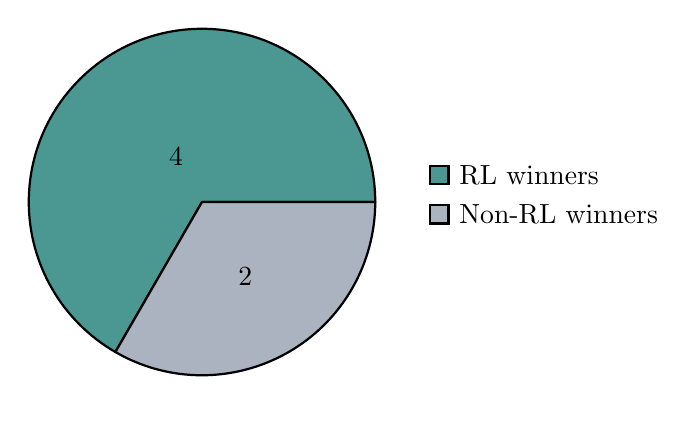
\begin{tikzpicture}
\pie[
    text=legend,
    radius=2.2,
    color={teal!75,slate!55},
    sum=auto,
    before number=,
    after number=
]{4/RL winners,2/Non-RL winners}
\end{tikzpicture}
\caption{Latency winner family split across six system-scenario comparisons}
\end{subfigure}
\hfill
\begin{subfigure}[t]{0.46\textwidth}
\centering
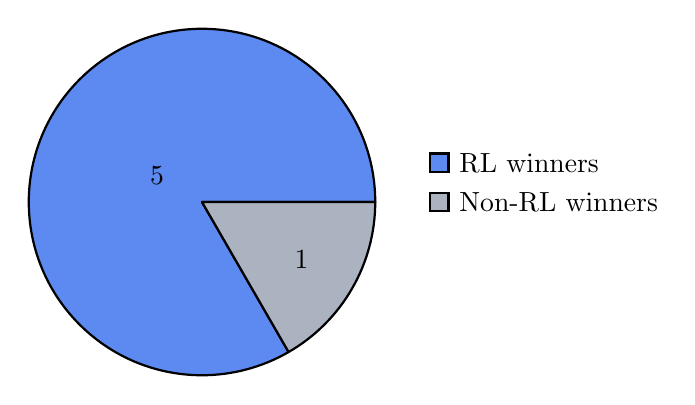
\begin{tikzpicture}
\pie[
    text=legend,
    radius=2.2,
    color={blueaccent!75,slate!55},
    sum=auto,
    before number=,
    after number=
]{5/RL winners,1/Non-RL winners}
\end{tikzpicture}
\caption{QPS winner family split across six system-scenario comparisons}
\end{subfigure}
\caption{Across the six system-scenario cases, RL methods win more often on both latency and throughput, but non-RL methods still win in some cases.}
\end{figure}

\section{Policy win counts}
\begin{figure}[H]
\centering
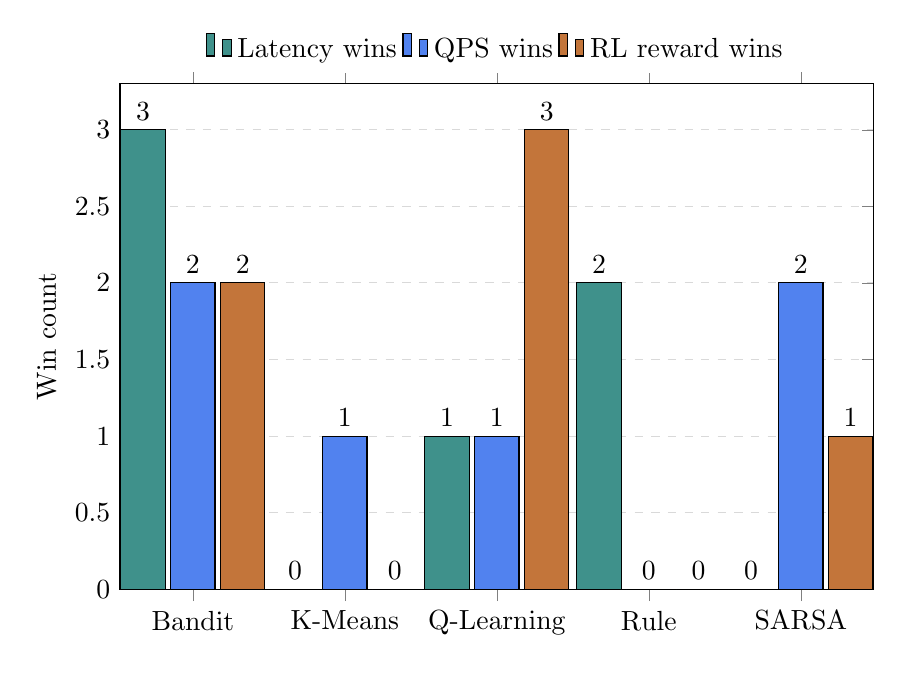
\begin{tikzpicture}
\begin{axis}[
    ybar,
    bar width=16pt,
    width=0.92\textwidth,
    height=8cm,
    ymin=0,
    ylabel={Win count},
    symbolic x coords={Bandit,K-Means,Q-Learning,Rule,SARSA},
    xtick=data,
    enlarge x limits=0.12,
    nodes near coords,
    nodes near coords align={vertical},
    legend style={at={(0.5,1.02)},anchor=south,legend columns=3,draw=none},
    ymajorgrids=true,
    grid style={dashed,gray!30}
]
\addplot[fill=teal!80] coordinates {(Bandit,3) (K-Means,0) (Q-Learning,1) (Rule,2) (SARSA,0)};
\addplot[fill=blueaccent!80] coordinates {(Bandit,2) (K-Means,1) (Q-Learning,1) (Rule,0) (SARSA,2)};
\addplot[fill=amber!80] coordinates {(Bandit,2) (K-Means,0) (Q-Learning,3) (Rule,0) (SARSA,1)};
\legend{Latency wins,QPS wins,RL reward wins}
\end{axis}
\end{tikzpicture}
\caption{Aggregate win counts across all systems and both scenarios. Latency and QPS wins use all five policies. Reward wins are reported only for RL methods.}
\end{figure}

\section{Interpretation of the cross-system summary}
The aggregate view already makes the main result visible. RL methods win most of the latency and QPS comparisons across the three applications. However, the policy that wins is not the same in every system. \QL{} dominates \TT{}, \Rule{} wins the clearest latency comparisons in \TS{}, and \Bandit{} is strongest on \SP{}. This is the strongest defensible answer to RQ1: RL is competitive and often strong, but the winner depends on the application.

\chapter{Per-System Results}
\section{Train-Ticket}
\subsection{Interpretation}
\TT{} provides the strongest evidence set in the study. Policy windows are numerous, zero-window counts are absent, and the runtime behavior is stable enough to support a stronger claim than in the other two systems. On this application, \QL{} is the best overall controller. It wins the faulted latency comparison and the faulted QPS comparison while also leading the RL family on reward in both healthy and faulted conditions. \SARSA{} reaches the highest healthy QPS, but its overall profile is less compelling than Q-Learning's.

\begin{figure}[H]
\centering
\begin{subfigure}[t]{0.48\textwidth}
\centering
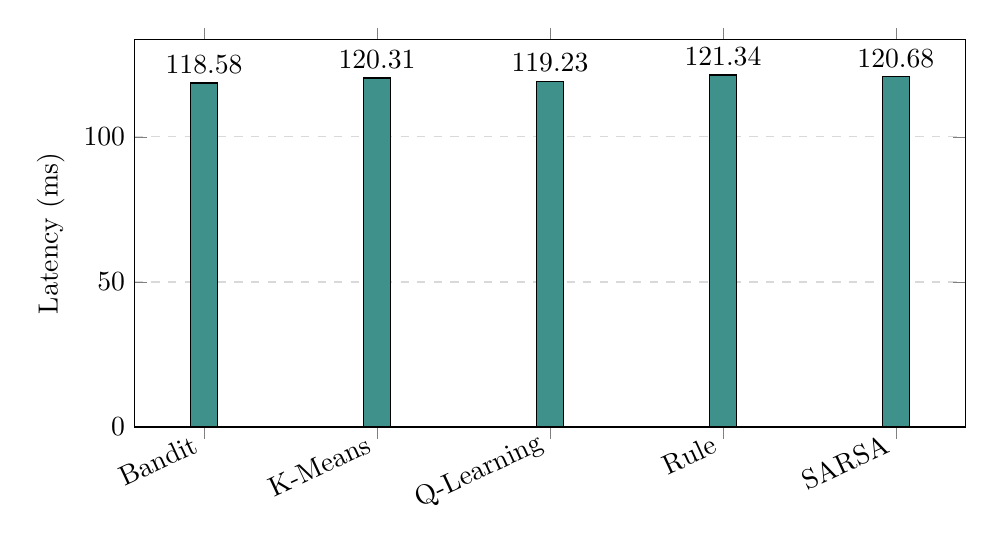
\begin{tikzpicture}
\begin{axis}[
    ybar,
    width=\textwidth,
    height=6.5cm,
    ymin=0,
    ylabel={Latency (ms)},
    symbolic x coords={Bandit,K-Means,Q-Learning,Rule,SARSA},
    xtick=data,
    x tick label style={rotate=25,anchor=east},
    ymajorgrids=true,
    grid style={dashed,gray!30},
    nodes near coords,
    nodes near coords align={vertical}
]
\addplot[fill=teal!80] coordinates {(Bandit,118.58) (K-Means,120.31) (Q-Learning,119.23) (Rule,121.34) (SARSA,120.68)};
\end{axis}
\end{tikzpicture}
\caption{Healthy latency}
\end{subfigure}
\hfill
\begin{subfigure}[t]{0.48\textwidth}
\centering
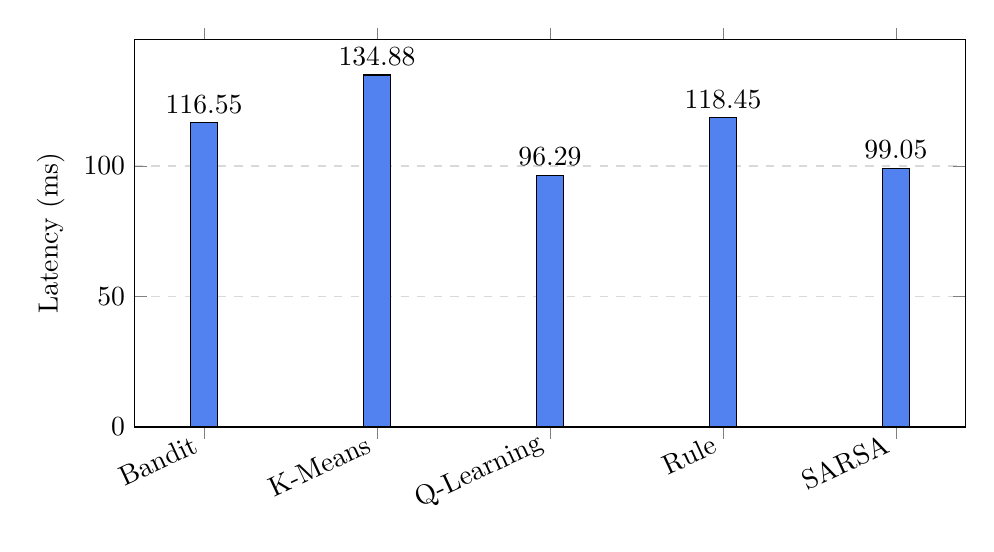
\begin{tikzpicture}
\begin{axis}[
    ybar,
    width=\textwidth,
    height=6.5cm,
    ymin=0,
    ylabel={Latency (ms)},
    symbolic x coords={Bandit,K-Means,Q-Learning,Rule,SARSA},
    xtick=data,
    x tick label style={rotate=25,anchor=east},
    ymajorgrids=true,
    grid style={dashed,gray!30},
    nodes near coords,
    nodes near coords align={vertical}
]
\addplot[fill=blueaccent!80] coordinates {(Bandit,116.55) (K-Means,134.88) (Q-Learning,96.29) (Rule,118.45) (SARSA,99.05)};
\end{axis}
\end{tikzpicture}
\caption{Faulted latency}
\end{subfigure}
\caption{\TT{} latency comparison. Lower is better.}
\end{figure}

\begin{figure}[H]
\centering
\begin{subfigure}[t]{0.48\textwidth}
\centering
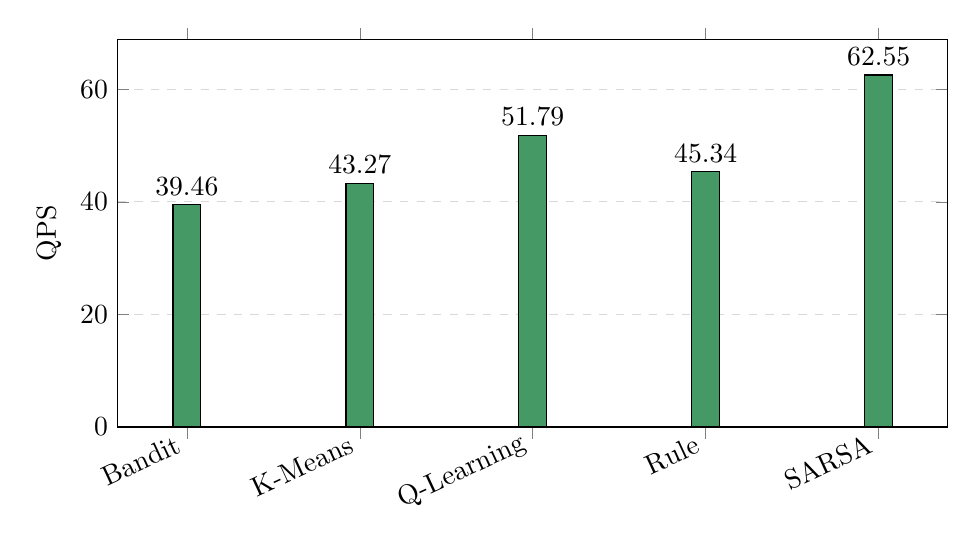
\begin{tikzpicture}
\begin{axis}[
    ybar,
    width=\textwidth,
    height=6.5cm,
    ymin=0,
    ylabel={QPS},
    symbolic x coords={Bandit,K-Means,Q-Learning,Rule,SARSA},
    xtick=data,
    x tick label style={rotate=25,anchor=east},
    ymajorgrids=true,
    grid style={dashed,gray!30},
    nodes near coords,
    nodes near coords align={vertical}
]
\addplot[fill=greenaccent!80] coordinates {(Bandit,39.464) (K-Means,43.268) (Q-Learning,51.793) (Rule,45.337) (SARSA,62.551)};
\end{axis}
\end{tikzpicture}
\caption{Healthy QPS}
\end{subfigure}
\hfill
\begin{subfigure}[t]{0.48\textwidth}
\centering
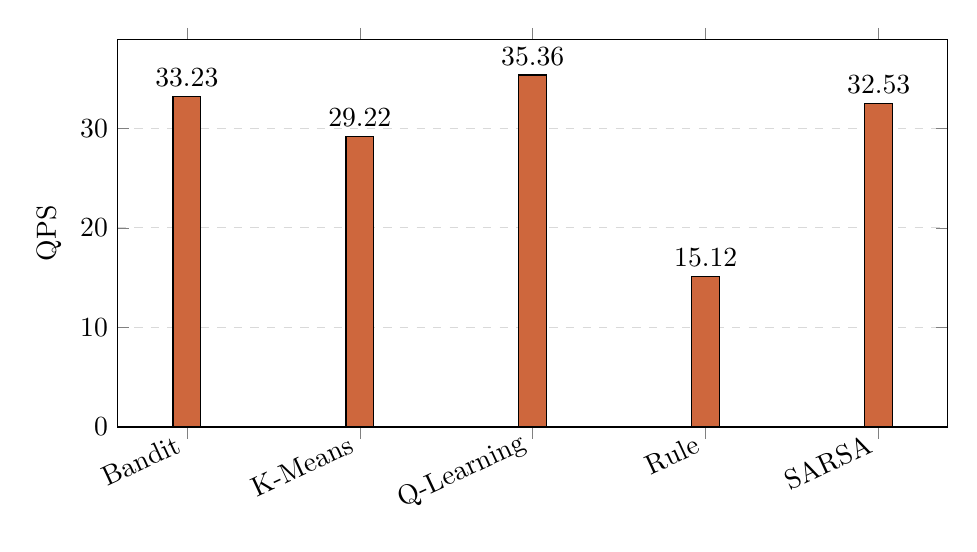
\begin{tikzpicture}
\begin{axis}[
    ybar,
    width=\textwidth,
    height=6.5cm,
    ymin=0,
    ylabel={QPS},
    symbolic x coords={Bandit,K-Means,Q-Learning,Rule,SARSA},
    xtick=data,
    x tick label style={rotate=25,anchor=east},
    ymajorgrids=true,
    grid style={dashed,gray!30},
    nodes near coords,
    nodes near coords align={vertical}
]
\addplot[fill=sarsaorange!80] coordinates {(Bandit,33.226) (K-Means,29.219) (Q-Learning,35.360) (Rule,15.124) (SARSA,32.529)};
\end{axis}
\end{tikzpicture}
\caption{Faulted QPS}
\end{subfigure}
\caption{\TT{} throughput comparison. Higher is better.}
\end{figure}

\begin{table}[H]
\centering
\caption{\TT{} policy results}
\resizebox{\textwidth}{!}{%
\begin{tabular}{llrrrrrr}
\toprule
Scenario & Policy & Latency (ms) & QPS & Error Rate & Avg Reward & Avg Rate & Decisions \\
\midrule
Healthy & Bandit & 118.58 & 39.464 & 0.0000 & 0.0937 & 0.050 & 11 \\
Healthy & K-Means & 120.31 & 43.268 & 0.0000 & n/a & 0.100 & 11 \\
Healthy & Q-Learning & 119.23 & 51.793 & 0.0000 & 0.1031 & 0.050 & 11 \\
Healthy & Rule & 121.34 & 45.337 & 0.0000 & n/a & 0.050 & 11 \\
Healthy & SARSA & 120.68 & 62.551 & 0.0000 & 0.0760 & 0.077 & 145 \\
\midrule
Faulted & Bandit & 116.55 & 33.226 & 0.0000 & 0.0637 & 0.050 & 11 \\
Faulted & K-Means & 134.88 & 29.219 & 0.0000 & n/a & 0.100 & 11 \\
Faulted & Q-Learning & 96.29 & 35.360 & 0.0000 & 0.0767 & 0.055 & 11 \\
Faulted & Rule & 118.45 & 15.124 & 0.0000 & n/a & 0.050 & 10 \\
Faulted & SARSA & 99.05 & 32.529 & 0.0000 & 0.0034 & 0.118 & 11 \\
\bottomrule
\end{tabular}}
\end{table}

\section{Timescale OpenTelemetry Demo}
\subsection{Interpretation}
The \TS{} result set is valid and complete, but it should be interpreted more carefully than \TT{}. The application clearly separates policies on latency and QPS, yet the reward function is not a pure runtime-performance score. That matters because \QL{} leads RL reward in the faulted case, but not in the final latency comparison. The most defensible statement for this application is therefore that \Rule{} is the strongest final-latency controller, while the RL family remains competitive and offers alternative throughput trade-offs.

\begin{figure}[H]
\centering
\begin{subfigure}[t]{0.48\textwidth}
\centering
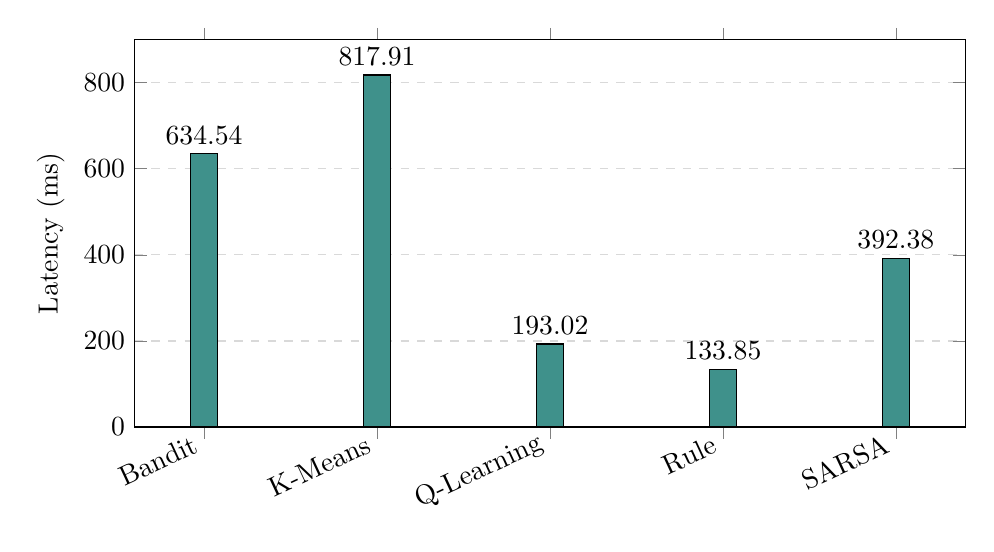
\begin{tikzpicture}
\begin{axis}[
    ybar,
    width=\textwidth,
    height=6.5cm,
    ymin=0,
    ylabel={Latency (ms)},
    symbolic x coords={Bandit,K-Means,Q-Learning,Rule,SARSA},
    xtick=data,
    x tick label style={rotate=25,anchor=east},
    ymajorgrids=true,
    grid style={dashed,gray!30},
    nodes near coords,
    nodes near coords align={vertical}
]
\addplot[fill=teal!80] coordinates {(Bandit,634.54) (K-Means,817.91) (Q-Learning,193.02) (Rule,133.85) (SARSA,392.38)};
\end{axis}
\end{tikzpicture}
\caption{Healthy latency}
\end{subfigure}
\hfill
\begin{subfigure}[t]{0.48\textwidth}
\centering
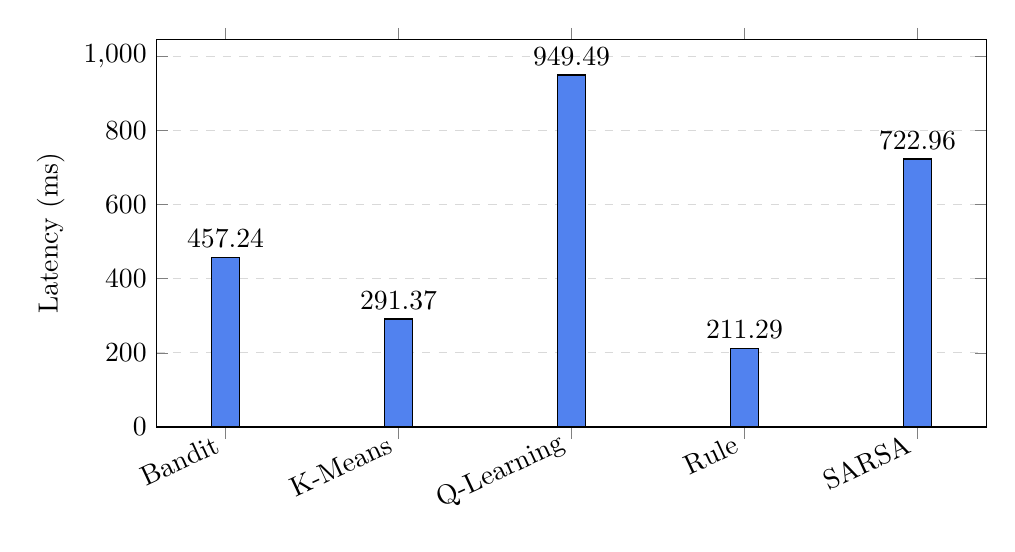
\begin{tikzpicture}
\begin{axis}[
    ybar,
    width=\textwidth,
    height=6.5cm,
    ymin=0,
    ylabel={Latency (ms)},
    symbolic x coords={Bandit,K-Means,Q-Learning,Rule,SARSA},
    xtick=data,
    x tick label style={rotate=25,anchor=east},
    ymajorgrids=true,
    grid style={dashed,gray!30},
    nodes near coords,
    nodes near coords align={vertical}
]
\addplot[fill=blueaccent!80] coordinates {(Bandit,457.24) (K-Means,291.37) (Q-Learning,949.49) (Rule,211.29) (SARSA,722.96)};
\end{axis}
\end{tikzpicture}
\caption{Faulted latency}
\end{subfigure}
\caption{\TS{} latency comparison. Lower is better.}
\end{figure}

\begin{figure}[H]
\centering
\begin{subfigure}[t]{0.48\textwidth}
\centering
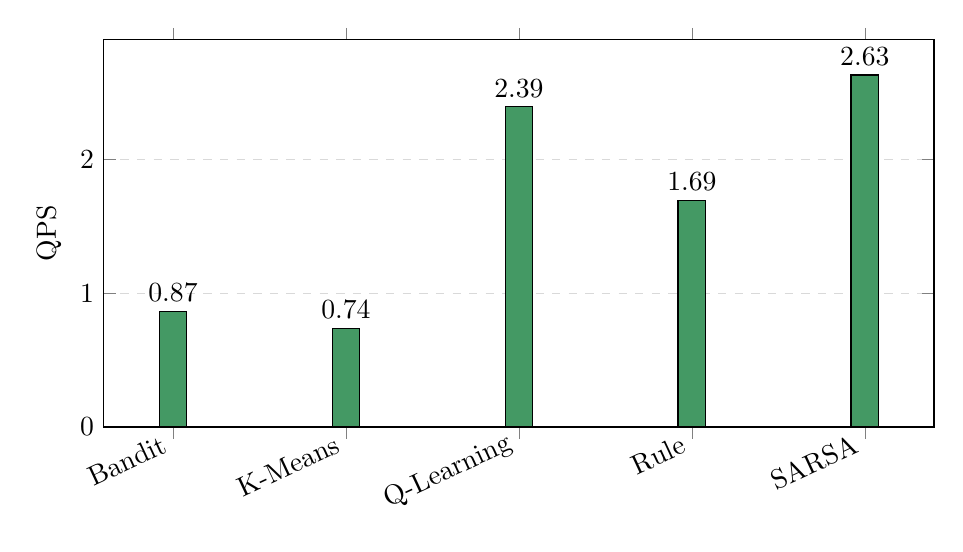
\begin{tikzpicture}
\begin{axis}[
    ybar,
    width=\textwidth,
    height=6.5cm,
    ymin=0,
    ylabel={QPS},
    symbolic x coords={Bandit,K-Means,Q-Learning,Rule,SARSA},
    xtick=data,
    x tick label style={rotate=25,anchor=east},
    ymajorgrids=true,
    grid style={dashed,gray!30},
    nodes near coords,
    nodes near coords align={vertical}
]
\addplot[fill=greenaccent!80] coordinates {(Bandit,0.865) (K-Means,0.736) (Q-Learning,2.392) (Rule,1.693) (SARSA,2.630)};
\end{axis}
\end{tikzpicture}
\caption{Healthy QPS}
\end{subfigure}
\hfill
\begin{subfigure}[t]{0.48\textwidth}
\centering
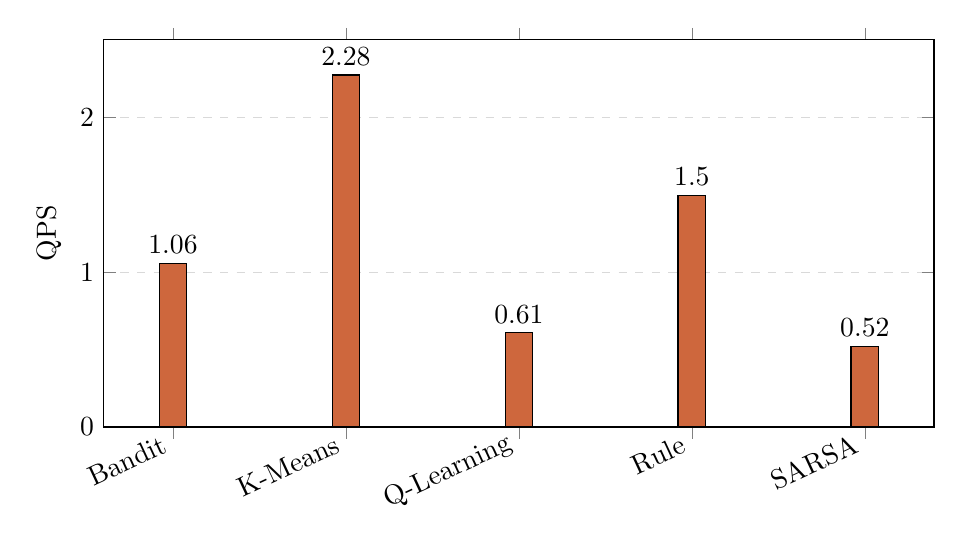
\begin{tikzpicture}
\begin{axis}[
    ybar,
    width=\textwidth,
    height=6.5cm,
    ymin=0,
    ylabel={QPS},
    symbolic x coords={Bandit,K-Means,Q-Learning,Rule,SARSA},
    xtick=data,
    x tick label style={rotate=25,anchor=east},
    ymajorgrids=true,
    grid style={dashed,gray!30},
    nodes near coords,
    nodes near coords align={vertical}
]
\addplot[fill=sarsaorange!80] coordinates {(Bandit,1.055) (K-Means,2.275) (Q-Learning,0.609) (Rule,1.495) (SARSA,0.523)};
\end{axis}
\end{tikzpicture}
\caption{Faulted QPS}
\end{subfigure}
\caption{\TS{} throughput comparison. Higher is better.}
\end{figure}

\begin{table}[H]
\centering
\caption{\TS{} policy results}
\resizebox{\textwidth}{!}{%
\begin{tabular}{llrrrrrr}
\toprule
Scenario & Policy & Latency (ms) & QPS & Error Rate & Avg Reward & Avg Rate & Decisions \\
\midrule
Healthy & Bandit & 634.54 & 0.865 & 0.0000 & 0.3129 & 0.050 & 4 \\
Healthy & K-Means & 817.91 & 0.736 & 0.0377 & n/a & 0.100 & 4 \\
Healthy & Q-Learning & 193.02 & 2.392 & 0.0000 & 0.2628 & 0.050 & 4 \\
Healthy & Rule & 133.85 & 1.693 & 0.0000 & n/a & 0.050 & 4 \\
Healthy & SARSA & 392.38 & 2.630 & 0.0195 & 0.3706 & 0.163 & 4 \\
\midrule
Faulted & Bandit & 457.24 & 1.055 & 0.0132 & 0.3164 & 0.050 & 4 \\
Faulted & K-Means & 291.37 & 2.275 & 0.0244 & n/a & 0.100 & 4 \\
Faulted & Q-Learning & 949.49 & 0.609 & 0.0152 & 0.5073 & 0.050 & 4 \\
Faulted & Rule & 211.29 & 1.495 & 0.0135 & n/a & 0.050 & 4 \\
Faulted & SARSA & 722.96 & 0.523 & 0.0169 & 0.4356 & 0.050 & 4 \\
\bottomrule
\end{tabular}}
\end{table}

\section{Spring Petclinic Microservices}
\subsection{Interpretation}
\SP{} is the third and final application. It contributes real business-domain microservice behavior, but its experimental evidence is weaker than \TT{} and \TS{} because the policy runs are shorter, some windows are sparse, and the degraded scenario falls back to heavier traffic when built-in chaos endpoints are unavailable. Even with those limitations, the final metrics are still interpretable. The strongest result on this application comes from \Bandit{}, which achieves the best final latency and the best throughput in both healthy and faulted conditions.

\begin{figure}[H]
\centering
\begin{subfigure}[t]{0.48\textwidth}
\centering
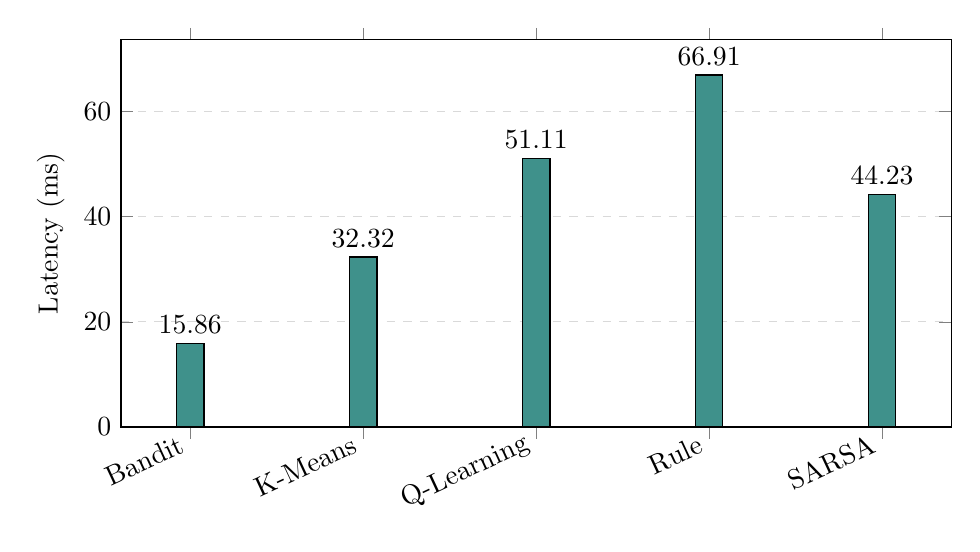
\begin{tikzpicture}
\begin{axis}[
    ybar,
    width=\textwidth,
    height=6.5cm,
    ymin=0,
    ylabel={Latency (ms)},
    symbolic x coords={Bandit,K-Means,Q-Learning,Rule,SARSA},
    xtick=data,
    x tick label style={rotate=25,anchor=east},
    ymajorgrids=true,
    grid style={dashed,gray!30},
    nodes near coords,
    nodes near coords align={vertical}
]
\addplot[fill=teal!80] coordinates {(Bandit,15.86) (K-Means,32.32) (Q-Learning,51.11) (Rule,66.91) (SARSA,44.23)};
\end{axis}
\end{tikzpicture}
\caption{Healthy latency}
\end{subfigure}
\hfill
\begin{subfigure}[t]{0.48\textwidth}
\centering
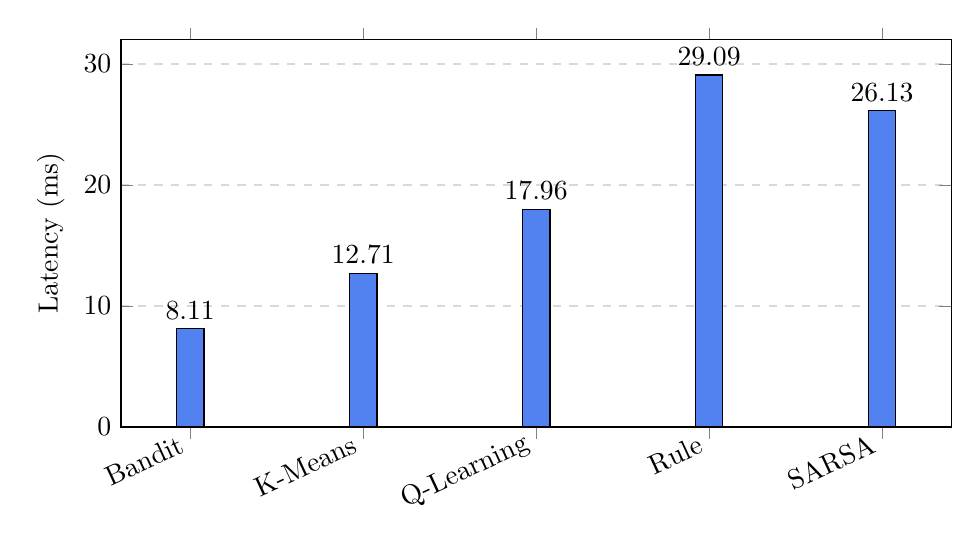
\begin{tikzpicture}
\begin{axis}[
    ybar,
    width=\textwidth,
    height=6.5cm,
    ymin=0,
    ylabel={Latency (ms)},
    symbolic x coords={Bandit,K-Means,Q-Learning,Rule,SARSA},
    xtick=data,
    x tick label style={rotate=25,anchor=east},
    ymajorgrids=true,
    grid style={dashed,gray!30},
    nodes near coords,
    nodes near coords align={vertical}
]
\addplot[fill=blueaccent!80] coordinates {(Bandit,8.11) (K-Means,12.71) (Q-Learning,17.96) (Rule,29.09) (SARSA,26.13)};
\end{axis}
\end{tikzpicture}
\caption{Faulted latency}
\end{subfigure}
\caption{\SP{} latency comparison. Lower is better.}
\end{figure}

\begin{figure}[H]
\centering
\begin{subfigure}[t]{0.48\textwidth}
\centering
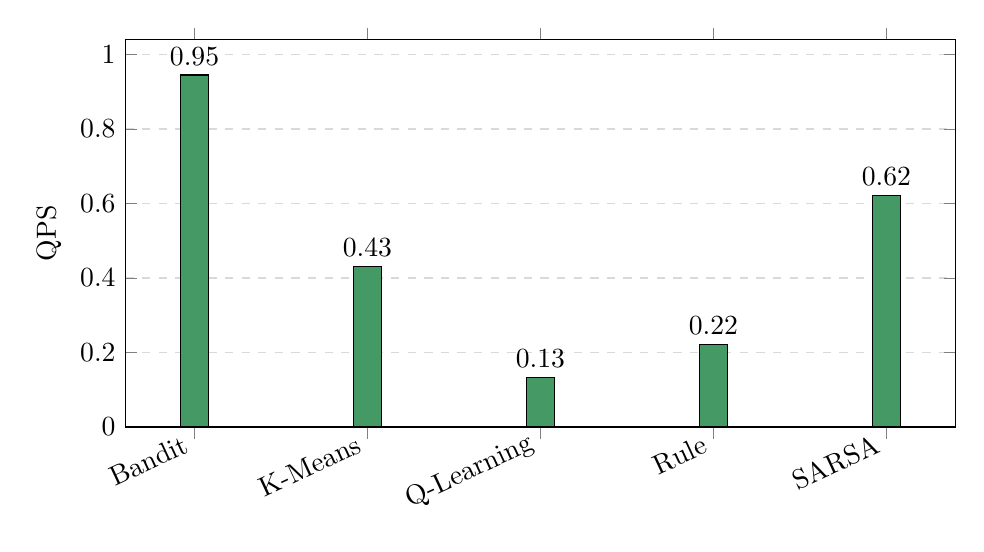
\begin{tikzpicture}
\begin{axis}[
    ybar,
    width=\textwidth,
    height=6.5cm,
    ymin=0,
    ylabel={QPS},
    symbolic x coords={Bandit,K-Means,Q-Learning,Rule,SARSA},
    xtick=data,
    x tick label style={rotate=25,anchor=east},
    ymajorgrids=true,
    grid style={dashed,gray!30},
    nodes near coords,
    nodes near coords align={vertical}
]
\addplot[fill=greenaccent!80] coordinates {(Bandit,0.945) (K-Means,0.432) (Q-Learning,0.133) (Rule,0.222) (SARSA,0.622)};
\end{axis}
\end{tikzpicture}
\caption{Healthy QPS}
\end{subfigure}
\hfill
\begin{subfigure}[t]{0.48\textwidth}
\centering
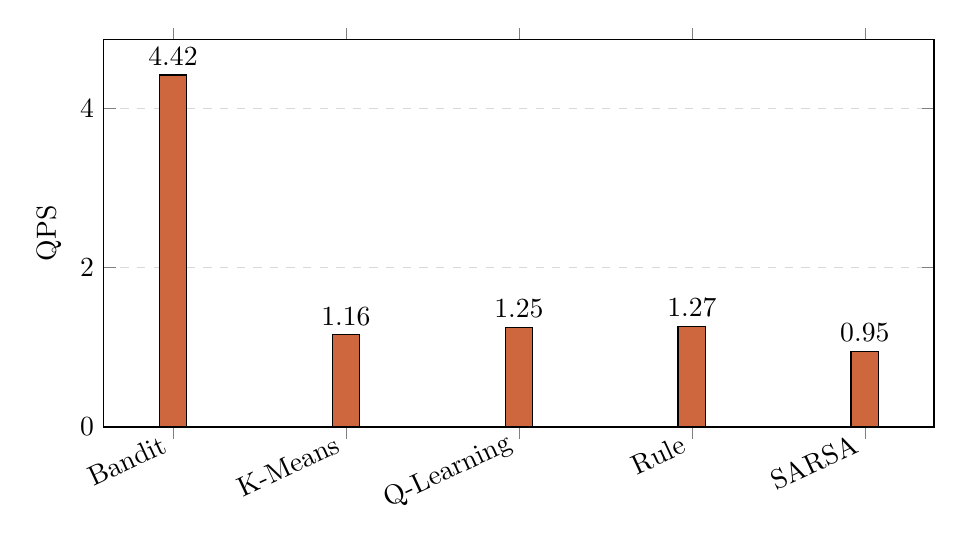
\begin{tikzpicture}
\begin{axis}[
    ybar,
    width=\textwidth,
    height=6.5cm,
    ymin=0,
    ylabel={QPS},
    symbolic x coords={Bandit,K-Means,Q-Learning,Rule,SARSA},
    xtick=data,
    x tick label style={rotate=25,anchor=east},
    ymajorgrids=true,
    grid style={dashed,gray!30},
    nodes near coords,
    nodes near coords align={vertical}
]
\addplot[fill=sarsaorange!80] coordinates {(Bandit,4.418) (K-Means,1.156) (Q-Learning,1.250) (Rule,1.267) (SARSA,0.945)};
\end{axis}
\end{tikzpicture}
\caption{Faulted QPS}
\end{subfigure}
\caption{\SP{} throughput comparison. Higher is better.}
\end{figure}

\begin{table}[H]
\centering
\caption{\SP{} policy results}
\resizebox{\textwidth}{!}{%
\begin{tabular}{llrrrrrrr}
\toprule
Scenario & Policy & Latency (ms) & QPS & Error Rate & Avg Reward & Avg Rate & Decisions & Zero Windows \\
\midrule
Healthy & Bandit & 15.86 & 0.945 & 0.1928 & 0.2105 & 0.125 & 2 & 0 \\
Healthy & K-Means & 32.32 & 0.432 & 0.0000 & -0.0838 & 0.100 & 1 & 0 \\
Healthy & Q-Learning & 51.11 & 0.133 & 0.0000 & 0.1110 & 0.075 & 2 & 0 \\
Healthy & Rule & 66.91 & 0.222 & 0.0000 & 0.0090 & 0.075 & 2 & 1 \\
Healthy & SARSA & 44.23 & 0.622 & 0.0000 & 0.0962 & 0.050 & 2 & 0 \\
\midrule
Faulted & Bandit & 8.11 & 4.418 & 0.2555 & 1.3779 & 0.050 & 2 & 1 \\
Faulted & K-Means & 12.71 & 1.156 & 0.0000 & 0.2148 & 0.100 & 2 & 0 \\
Faulted & Q-Learning & 17.96 & 1.250 & 0.0000 & 0.0823 & 0.075 & 2 & 0 \\
Faulted & Rule & 29.09 & 1.267 & 0.0880 & -0.1621 & 0.650 & 2 & 0 \\
Faulted & SARSA & 26.13 & 0.945 & 0.1661 & 1.2431 & 0.050 & 2 & 0 \\
\bottomrule
\end{tabular}}
\end{table}

\chapter{Integrated Interpretation and Answer to RQ1}
\section{Main synthesis}
The three applications do not support the claim that one controller is universally best. Instead, they support a stronger and more realistic claim:
\begin{quote}
\textbf{RL-based adaptive tracing is a credible and often high-performing choice, but its advantage is system-dependent rather than universal.}
\end{quote}
This claim is stronger because it survives cross-system comparison instead of depending on a single benchmark.

\section{What the three systems show together}
\begin{itemize}
    \item On \TT{}, \QL{} is the strongest overall controller. This is the clearest RL win in the study.
    \item On \TS{}, \Rule{} wins the most defensible final-latency comparisons, while RL remains competitive on some throughput and reward views.
    \item On \SP{}, \Bandit{} is the strongest final-runtime controller, especially on latency and throughput.
\end{itemize}
The systems therefore disagree on the identity of the best controller, but they agree on something more important: adaptive tracing quality is not random, and method choice matters.

\section{How reward should be interpreted}
Reward should not be treated identically across the three applications. In \TT{}, reward aligns reasonably well with runtime performance. In \TS{}, reward must be interpreted carefully because the reward design is not a pure runtime-performance objective. In \SP{}, reward is available and useful, but the runs are short and the decision count is low. For that reason, the final cross-system synthesis gives primary weight to latency, QPS, error rate, and run quality, and uses reward as supporting evidence.

\section{Evidence quality is not equal across the systems}
The strength of evidence differs across the applications:
\begin{itemize}
    \item \TT{} is the strongest evidence set. It has the highest stability and the most defensible policy comparison.
    \item \TS{} is valid and useful, but the reward caveat weakens any claim that depends only on average reward.
    \item \SP{} is complete, but the low decision counts and occasional sparse windows make it the weakest of the three result sets.
\end{itemize}
This means the most confident project-level claim is not ``RL always wins''. The most confident claim is that RL methods are competitive and often strong, but system-specific behavior remains decisive.

\section{Final answer to RQ1}
The final answer to RQ1 across all three applications is:

\begin{quote}
\textbf{RL-based adaptive tracing performs competitively against non-RL baselines and often achieves the best result, but there is no universal winner across all systems. Q-Learning is strongest on Train-Ticket, Rule is strongest on the Timescale OpenTelemetry Demo, and Bandit is strongest on Spring Petclinic Microservices.}
\end{quote}

This is the correct conclusion because it reflects the actual experimental evidence instead of forcing a single algorithmic winner across incompatible application contexts.

\chapter{Limitations and Next Steps}
\begin{itemize}
    \item \textbf{Reward symmetry is imperfect.} Non-RL methods do not expose reward in the same way as RL methods, and one application has a reward-design caveat.
    \item \textbf{Fault models differ across applications.} This is acceptable for RQ1, but it means the comparison is per-application rather than a single synthetic fault across all systems.
    \item \textbf{Run quality varies by application.} \TT{} is the strongest evidence set; \TS{} and \SP{} are valid but less stable.
    \item \textbf{Longer repeated trials would strengthen the final claims.} This is especially important for \SP{}, where the decision count is low.
\end{itemize}
The next logical step is not another one-off comparison. It is either repeated trials to tighten statistical confidence or a shift to later research questions that examine robustness under more varied runtime changes.

\appendix
\chapter{Source Reports and Artifacts}
The LaTeX report consolidates the following final per-system HTML reports and their underlying experiment results:
\begin{itemize}
    \item \texttt{/Users/dan/train-ticket-python/reports/final report/rq1\_full\_report.html}
    \item \texttt{/Users/dan/timescale-otel-demo/reports/rq1\_timescale\_otel\_demo\_report.html}
    \item \texttt{/Users/dan/spring-petclinic-microservices/reports/rq1\_spring\_petclinic\_microservices\_report.html}
    \item Consolidated HTML report: \texttt{/Users/dan/rq1\_all\_three\_systems\_report.html}
\end{itemize}

\end{document}
